\documentclass[11pt]{article}
\usepackage[margin=1in]{geometry}
\usepackage{amsmath,amssymb,amsthm,mathtools}
\usepackage{graphicx}
\usepackage[hidelinks]{hyperref}
\usepackage{microtype}

\newtheorem{theorem}{Theorem}
\newtheorem{lemma}{Lemma}
\newcommand{\R}{\mathbb R}
\newcommand{\cD}{\mathcal D}
\newcommand{\cP}{\mathcal P}

\title{All real phase-retrieving dual frames are generic}
\author{Automated mathematics run \texttt{fa\_banach\_001}}
\date{11 August 2026}

\begin{document}
\maketitle

\begin{center}
\fbox{\parbox{0.91\textwidth}{\textbf{Status.}
Candidate partial result, likely valid.  The real finite-dimensional theorem
is complete; the complex case remains open.}}
\end{center}

\begin{abstract}
Given a finite real phase-retrieving frame with arbitrary redundancy, we prove
that its phase-retrieving duals form a relatively Zariski-open, Euclidean-open
dense, full-measure subset of the affine space of all duals.  We give a single
explicit polynomial that classifies these duals.  Moreover, on the line from
any dual to the canonical dual, all but finitely many points do phase
retrieval.  This removes the source theorem's minimal-length restriction
$m=2n-1$.
\end{abstract}

\section{Source question and source limitation}

Arabyani-Neyshaburi, Arefijamaal, and Kamyabi-Gol ask whether the
phase-retrieving duals of a phase-retrieving frame can be classified and
whether they are dense among all duals \cite{source}.  The same abstract says
that their results establish density only for some frame classes.

\begin{center}

\includegraphics[width=\textwidth]{figures/open_problem_crop.png}
\end{center}

Their main real density result, Theorem 2.3, treats a frame of exactly
$2n-1$ vectors in $\R^n$.

\begin{center}
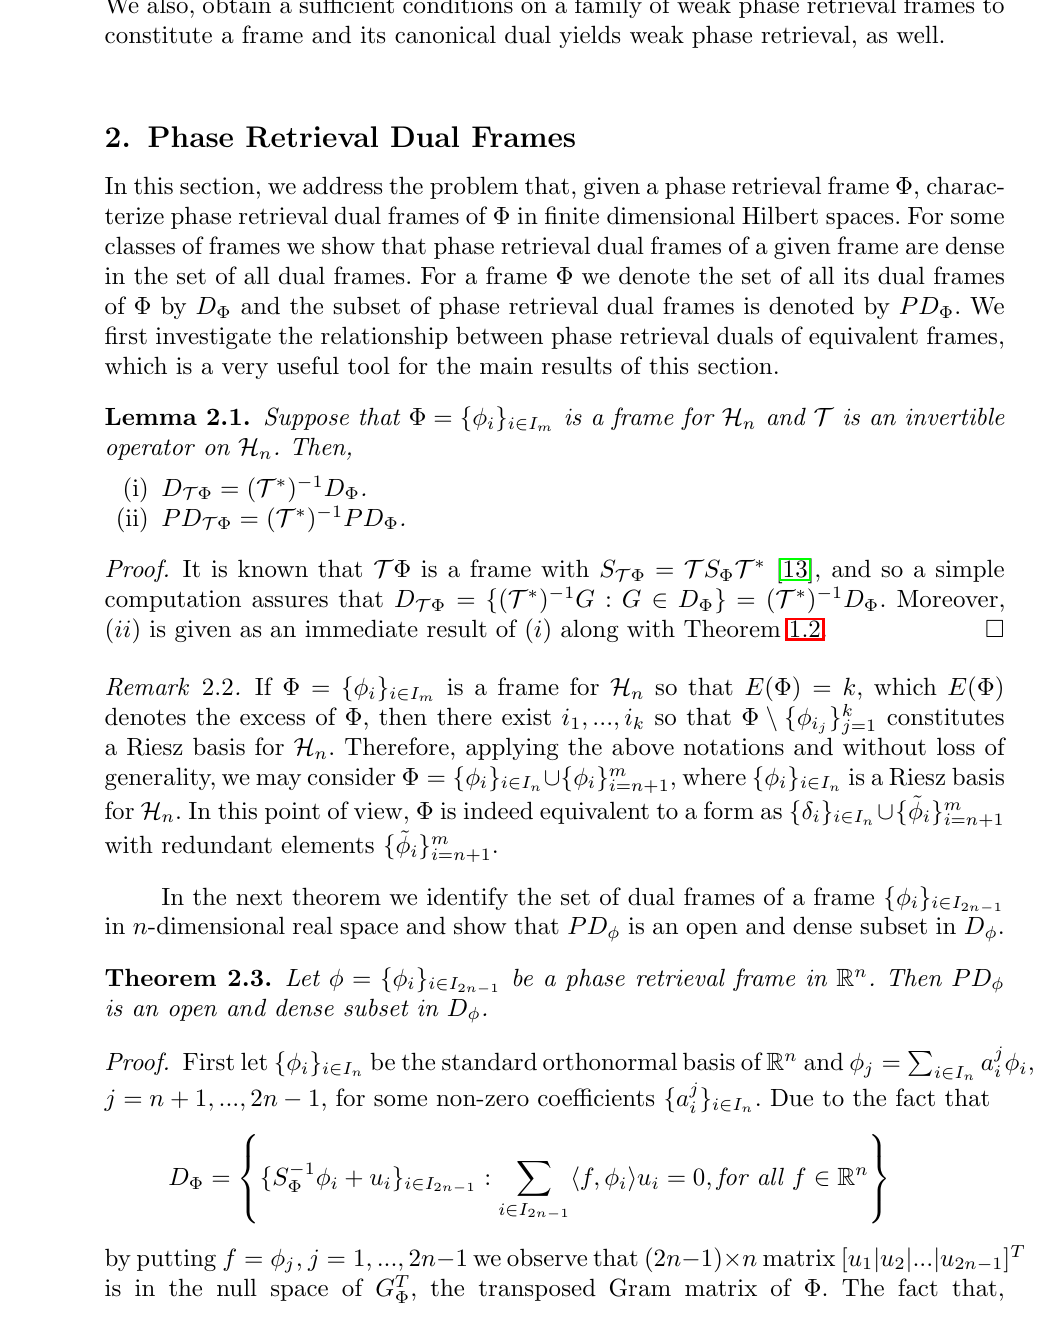
\includegraphics[width=\textwidth]{figures/source_minimal_length_theorem_crop.png}
\end{center}

The result below covers every finite real phase-retrieving frame, with no
restriction on its redundancy, and supplies an explicit classification
polynomial.  It does not address complex frames.

\section{Definitions}

Let $\Phi=(\phi_i)_{i=1}^m\subset\R^n$ be a frame and let
$F=[\phi_1\ \cdots\ \phi_m]\in\R^{n\times m}$ be its synthesis matrix.  A
frame $G=(g_i)_{i=1}^m$, with synthesis matrix again denoted $G$, is a dual of
$\Phi$ when
\begin{equation}\label{eq:dual-affine}
 GF^T=I_n.
\end{equation}
Thus the dual space
\[
 \cD_\Phi=\{G\in\R^{n\times m}:GF^T=I_n\}
\]
is a nonempty affine subspace.  Its canonical point is
\begin{equation}\label{eq:canonical}
 G_0=S_\Phi^{-1}F,\qquad S_\Phi=FF^T.
\end{equation}

A real frame $G$ does phase retrieval when
\[
 |\langle x,g_i\rangle|=|\langle y,g_i\rangle|\quad(1\le i\le m)
 \quad\Longrightarrow\quad x=\pm y.
\]
Write $\cP\cD_\Phi$ for the phase-retrieving members of $\cD_\Phi$.

For $I\subseteq[m]$, define
\begin{equation}\label{eq:RI}
 R_I(G)=\sum_{\substack{J\subseteq I\\|J|=n}}
 \det(G_J)^2,
\end{equation}
where $G_J$ is the $n\times n$ submatrix with columns in $J$; an empty sum is
zero.  Finally set
\begin{equation}\label{eq:P}
 P(G)=\prod_{I\subseteq[m]}\bigl(R_I(G)+R_{I^c}(G)\bigr).
\end{equation}

\section{Proof intuition}

The real complement-property theorem says that phase retrieval is exactly the
condition that, for each partition of the frame vectors, at least one side
spans.  A side spans precisely when at least one maximal minor is nonzero;
summing squares of all such minors turns this into one polynomial inequality.
Multiplying over all partitions gives \eqref{eq:P}.

The only way this algebraic certificate could fail to imply density in the
affine dual space would be if it vanished identically there.  The canonical
dual rules that out: it remains phase retrieving because its vectors are an
invertible self-adjoint image of the original phase-retrieving frame.  The
zero set of a nonzero polynomial is nowhere dense and null.  On a line toward
the canonical dual, the same polynomial becomes a nonzero univariate
polynomial, giving only finitely many exceptional points.

\section{Main theorem}

\begin{theorem}[Arbitrary real redundancy]\label{thm:main}
Let $\Phi=(\phi_i)_{i=1}^m$ be any finite phase-retrieving frame for $\R^n$.
Then
\begin{equation}\label{eq:classification}
 \cP\cD_\Phi=\{G\in\cD_\Phi:P(G)\ne0\},
\end{equation}
with $P$ given by \eqref{eq:P}.  Consequently $\cP\cD_\Phi$ is relatively
Zariski open, Euclidean open and dense in $\cD_\Phi$, and its complement has
Lebesgue measure zero in that affine space.

More strongly, for every $G\in\cD_\Phi$, let
\[
 G_t=(1-t)G+tG_0,
\]
where $G_0$ is the canonical dual.  Then $G_t$ is a phase-retrieving dual for
all real $t$ except a finite set.  In particular, every dual is a limit of
phase-retrieving duals lying on this line.
\end{theorem}

\begin{proof}
We use the real complement-property characterization of phase retrieval
\cite[Theorem~2.8]{BCE}; it is also restated as Theorem 1.4 of the source
paper \cite[p.~3]{source}.  It says that a real frame $G=(g_i)_{i=1}^m$ does
phase retrieval if and only if, for every $I\subseteq[m]$, either
\[
 \operatorname{span}\{g_i:i\in I\}=\R^n
 \quad\text{or}\quad
 \operatorname{span}\{g_i:i\in I^c\}=\R^n.
\]
By maximal-minor rank detection,
\[
 R_I(G)>0
 \quad\Longleftrightarrow\quad
 \operatorname{span}\{g_i:i\in I\}=\R^n.
\]
Every factor in \eqref{eq:P} is nonnegative.  Hence $P(G)\ne0$ exactly when
every partition has a spanning side.  This proves \eqref{eq:classification}.

Next, $G_0$ in \eqref{eq:canonical} is a dual by direct multiplication:
$G_0F^T=S_\Phi^{-1}FF^T=I_n$.  It also does phase retrieval.  Indeed,
if
\[
 |\langle x,S_\Phi^{-1}\phi_i\rangle|
 =|\langle y,S_\Phi^{-1}\phi_i\rangle|
 \quad\text{for every }i,
\]
self-adjointness of $S_\Phi^{-1}$ rewrites this as equality of the
$\Phi$-measurements of $S_\Phi^{-1}x$ and $S_\Phi^{-1}y$.  Since $\Phi$ does
phase retrieval,
$S_\Phi^{-1}x=\pm S_\Phi^{-1}y$, and invertibility gives $x=\pm y$.
Therefore $P(G_0)>0$.

The restriction of $P$ to the finite-dimensional affine space $\cD_\Phi$ is
thus a nonzero polynomial.  Its nonvanishing locus is relatively Zariski
open.  The zero set of a nonzero real polynomial has empty Euclidean interior
and Lebesgue measure zero, proving the asserted openness, density, and
full-measure statement.

Finally, \eqref{eq:dual-affine} shows that $G_t\in\cD_\Phi$ for every $t$.
The function
\[
 q_G(t)=P((1-t)G+tG_0)
\]
is a real polynomial, and $q_G(1)=P(G_0)>0$.  Thus $q_G$ is not identically
zero and has only finitely many real roots.  By
\eqref{eq:classification}, precisely those roots can fail phase retrieval.
Choosing nonroots tending to zero proves the last assertion.
\end{proof}

\section{Scope, verification, and novelty}

The proof is exact and has no computational dependency.  It upgrades source
Theorem 2.3 from $m=2n-1$ to arbitrary finite $m$ and adds an explicit global
classification, a full-measure conclusion, and radial finite-exception
genericity.  The complex case remains open because the real complement
property used above has no direct complex counterpart of this form.

A bounded search on 11 August 2026 checked the run indexes, the exact title,
and official arXiv API queries for ``phase retrieval dual frames,''
``alternate dual frames'' with ``phase retrieval,'' and ``dual frames'' with
``open and dense'' and ``phase retrieval.''  Each exact query returned only
arXiv:2301.05045v1.  No prior arbitrary-redundancy or radial theorem was
found.  Novelty is plausible, not an exhaustive certification.

\paragraph{Human-review recommendation.}
Check the equivalence between \eqref{eq:P} and the complement property and the
canonical-dual argument.  The remaining algebraic-topological consequences
are standard.

\begin{thebibliography}{9}

\bibitem{source}
F.~Arabyani-Neyshaburi, A.~A.~Arefijamaal, and R.~A.~Kamyabi-Gol,
\emph{Characterization of (weak) phase retrieval dual frames},
arXiv:2301.05045v1 (2023).

\bibitem{BCE}
R.~Balan, P.~G.~Casazza, and D.~Edidin,
\emph{On signal reconstruction without phase},
Appl. Comput. Harmon. Anal. 20 (2006), 345--356.

\end{thebibliography}

\end{document}

